% Se incluyen los paquetes.
% Clase del texto con el tamaño de la fuente.
\documentclass[11pt, twoside, letterpaper]{IEEEtran}

% Tamaño del papel y de las margenes
\usepackage{geometry}
\geometry{
    letterpaper,
    top=0.75in, 
    bottom=1in, 
    left=0.68in, 
    right=0.68in,
    marginparwidth=0.5in,
}

% Se selecciona el idioma y se redefine el termino "Cuadro" por Tabla y "Resumen" por Abstract.
\usepackage[spanish]{babel}
\renewcommand{\spanishtablename}{Tabla}
\renewcommand{\spanishabstractname}{Abstract}
\selectlanguage{spanish}

% Codificación a utilizar.
\usepackage[utf8]{inputenc}
\usepackage[T1]{fontenc}
\usepackage{lmodern}

% Se corrige silabas de algunas palabras.
\hyphenation{pa-la-bra pa-rra-fo}

% Para modificar el Titulo
\usepackage{titling}
\pretitle{} \posttitle{}
\preauthor{} \postauthor{}
\predate{} \postdate{}

% Se selecciona el directorio donde se encuentran las imágenes.
\usepackage{graphicx, wrapfig, float}
\graphicspath{{images/}}

% Para ajustar el interlineado.
\usepackage{setspace}

% Para ajustar la sangría de la primera linea.
\setlength{\parindent}{3em}

% Para ajustar el espacio entre párrafos.
\setlength{\parskip}{2ex}

% Paquetes matemáticos.
\usepackage{amssymb, amsmath, amsbsy, mathdots, mathrsfs, cancel}

% Para listas personalizadas.
\usepackage{enumitem}

% Para las letras capitales.
\usepackage{lettrine}

% Encabezado y pie de página

% Configuración de los encabezados y los pie de página.
\usepackage{fancyhdr}
\pagestyle{fancy}
\fancyhf{}
% Elementos en la cabecera [par]{impar}
\lhead[\thepage]{}
\chead[]{}
\rhead[]{\thepage}
\renewcommand{\headrulewidth}{0.0pt}

% Elementos en el pie de página [par]{impar}
\lfoot[]{}
\cfoot[]{}
\rfoot[]{}
% \renewcommand{\footrulewidth}{0.5pt}


% Primera página
\fancypagestyle{plain}{
    \fancyhead[L]{}
    \fancyhead[C]{}
    \fancyhead[R]{}
    \fancyfoot[L]{}
    \fancyfoot[C]{}
    \fancyfoot[R]{}
    \renewcommand{\headrulewidth}{0.0pt}
    %\renewcommand{\footrulewidth}{0.5pt}
}

% Textos de prueba.
\usepackage{blindtext}

% Enlaces.
\usepackage{hyperref}

% Paquete gráfico
\usepackage{tikz}

% Referencias.
\usepackage[maxbibnames=99, sorting=none, backend=biber, style=ieee]{biblatex}
\addbibresource{references.bib}

% Se incluye el titulo.
% Titulo.
\DeclareRobustCommand{\titlecontent}{
    % Contenido de la sección de titulo.
    \begin{center}
        \Huge \textbf{Implementación de un efecto sobre una imagen} \\  \hfill \break
        \large Práctica 1 \\  \hfill \break
    \end{center}
}

% Autores.
\DeclareRobustCommand{\authorcontent}{
    % Contenido de la sección de autores.
    \begin{center}
        \normalsize Ricardo Andrés Calvo Méndez, Jorge Aurelio Morales Manrique \\ \hfill \break
        \small \textit{Universidad Nacional de Colombia} \\
        \small \textit{Bogotá, Colombia}\\ \hfill \break
        \texttt{\href{mailto:rcalvom@unal.edu.co}{rcalvom@unal.edu.co}}\\
        \texttt{\href{mailto:jomorales@unal.edu.co}{jomorales@unal.edu.co}}\\
    \end{center}
}

% Fecha.
\DeclareRobustCommand{\datecontent}{
    % Contenido de la sección de fecha.
    \begin{center}
        \scriptsize \today \normalsize
    \end{center}
}

% Asignación de los comandos.
\title{\titlecontent}
\author{\authorcontent}
\date{\datecontent}

% Inicio del documento.
\begin{document}

% Creación del título.
\maketitle

% Abstract del articulo, si se desea omitir, comentar la siguiente linea.
\begin{abstract}
    Image processing is a method to perform some operations on an image, in order to get an enhanced image or to extract some useful information from it. This technique is related to the field of parallel computing in the sense that the filters used are highly parallelizable, the pixels transformations are independent of each other. The purpose of this practice is to apply a filter to images of different sizes and analize the response time and speedup using different numbers of threads.
\end{abstract}


\section{Introducción}
La computación paralela es un paradigma de cómputo en el cual múltiples cálculos o procesos son ejecutados simultáneamente. Problemas grandes pueden ser divididos en problemas más pequeños que pueden ser ejecutados en diferentes unidades lógicas del procesador para obtener tiempos de ejecución más bajos. La computación paralela es ampliamente usada en el campo de ``high performance computing'' gracias a las ventajas que ofrece en la ejecución de algoritmos que cumplen con la condición de ser paralelizables. Una de las aplicaciones más reconocidas es el procesamiento de imágenes, por medio de la aplicación de filtros basados en kernels, debido a que las operaciones realizadas sobre los píxeles son independientes entre si, lo que permite hacer una división del cómputo entre varios hilos. El objetivo de esta práctica es aplicar el filtro de detección de bordes sobre imágenes con resoluciones 720p, 1080p y 4k, por medio de una implementación en lenguaje C que haga uso de la librería ``pthread.h'' para la ejecución con múltiples hilos. Finalmente se realiza el respectivo análisis de tiempo de respuesta y speedup para cada uno de los casos.

\section{Diseño del programa}
La aplicación tiene 3 componentes principales:
\begin{itemize}
    \item \textbf{Script de Bash:} realiza la ejecución del algoritmo en C para cada una de las imágenes de prueba variando el número de hilos con valores de 1, 2, 4, 8 y 16. Al finalizar cada caso almacena el tiempo de ejecución en un archivo de texto plano. Una vez se obtienen los resultados para cada caso de prueba se ejecuta el script en Python para la generación de las gráficas y el reporte.
    \item \textbf{Script en Python:} realiza la lectura de los archivos de resultados, agrupando los valores por tipo de imagen, para luego, haciendo uso de la librería \textbf{matplotlib} generar las gráficas correspondientes al tiempo de respuesta y speedup para las imágenes con resolución 720p, 1080p y 4k. Así mismo, el script compila el reporte latex con la última versión de gráficas generadas.
    \item \textbf{Algoritmo en C:} contiene la implementación del filtro para detección de bordes el cual está descrito en el siguiente fragmento de pseudocódigo:
    \begin{figure}[H]
        \centering
        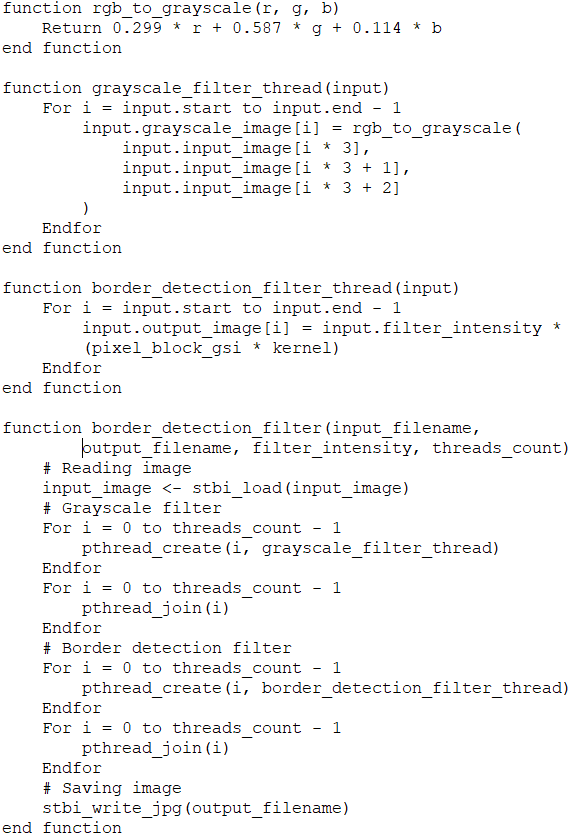
\includegraphics[width=0.4\textwidth]{../plots/pseudocode.PNG}
        \caption{Pseudocódigo algoritmo para detección de bordes}
    \end{figure}
    Las funciones ``rgb\_to\_grayscale'' y ``grayscale\_filter\_thread'' corresponden a la conversión de cada pixel de RGB a escala de grises, esto se realiza ya que para la detección de bordes no es necesario conocer los valores de color de los 3 canales, se requiere conocer la intensidad del pixel, por lo cual se usa la escala de grises. Las funciones ``border\_detection\_filter\_thread'' y ``border\_detection\_filter'' corresponden a la aplicación del filtro de detección de bordes para el cual el valor de cada pixel se calculo a través de una operación de convolución entre la matriz 3x3, que corresponde al pixel actual y sus vecinos, y el kernel el cual tiene los siguientes valores:
    \vspace{6mm}
    \begin{center}
        $\begin{pmatrix}
            -1 & -1 & -1\\
            -1 & 8 & -1\\
            -1 & -1 & -1
        \end{pmatrix}$
    \end{center}
    \newpage
    Las funciones para los filtros de escala de grises y detección de bordes son ejecutados utilizando múltiples hilos de acuerdo al argumento que indique el usuario. Para realizar la distribución de datos o balanceo de carga se utiliza el método blockwise (división de los datos en segmentos iguales), el cual se describe en el siguiente diagrama:
    \begin{figure}[H]
        \centering
        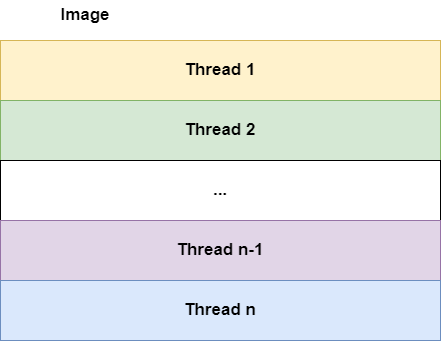
\includegraphics[width=0.4\textwidth]{../plots/load_balancing.drawio.png}
        \caption{Método blockwise para balanceo de carga}
    \end{figure}
\end{itemize}

\section{Experimentos}

Para la ejecución del programa, se han escogido 3 imágenes diferentes con tamaños 4k, 1080p y 720p; a cada una de las imágenes les será aplicado el filtro de detección de bordes usando ejecución secuencial y ejecuciones paralelas de 2, 4, 8 y 16. Combinando los tres tamaños de las imágenes y los cuatro tipos de ejecución, en total serán 12 casos de prueba.

Las siguientes son las imágenes a las cuales se les va a aplicar el filtro:

\begin{figure}[H]
    \centering
    
\includegraphics[width=0.4\textwidth]{../plots/4k.jpg}
    \caption{Miniatura de imagen con tamaño 4k que va a ser procesada}
\end{figure}

\begin{figure}[H]
    \centering
    
\includegraphics[width=0.4\textwidth]{../plots/1080p.jpg}
    \caption{Miniatura de imagen con tamaño 1080p que va a ser procesada}
\end{figure}

\begin{figure}[H]
    \centering
    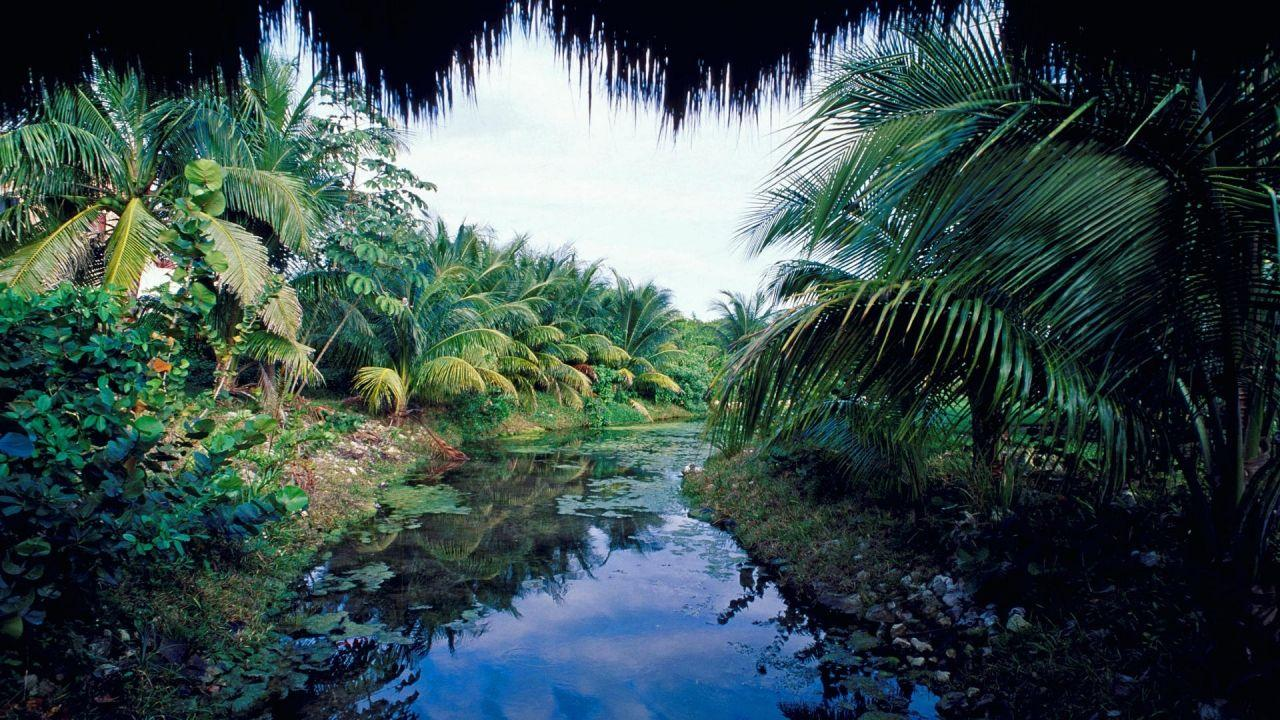
\includegraphics[width=0.4\textwidth]{../plots/720p.jpg}
    \caption{Miniatura de imagen con tamaño 720p que va a ser procesada}
\end{figure}

Para la automatización de la ejecución de los anteriores casos de prueba se utiliza el bash script \textit{execute\_script.sh} que ejecutará cada uno de los casos y almacenará los resultados en archivos de texto plano para su posterior análisis.

\section{Resultados}

Para la ejecución de los casos de prueba mencionados anteriormente se ha utilizado un procesador AMD Ryzen 5 4500U el cuál cuenta con 6 núcleos a 2.3 GHz de frecuencia de reloj.

Los resultados obtenidos de ejecutar el filtro en las 3 imágenes mencionadas anteriormente son los siguientes:

\subsection{Imagen de tamaño 4k}

La imagen obtenida de aplicar el filtro es la siguiente:

\begin{figure}[H]
    \centering
    \includegraphics[width=0.4\textwidth]{../plots/4k.out.jpg}
    \caption{Miniatura de imagen con tamaño 4k con el filtro de detección de bordes aplicado.}
\end{figure}

Las gráficas que resumen y comparan los tiempo de respuesta y los speed up de la aplicación del filtro a esta imagen son los siguientes:

\begin{figure}[H]
    \centering
    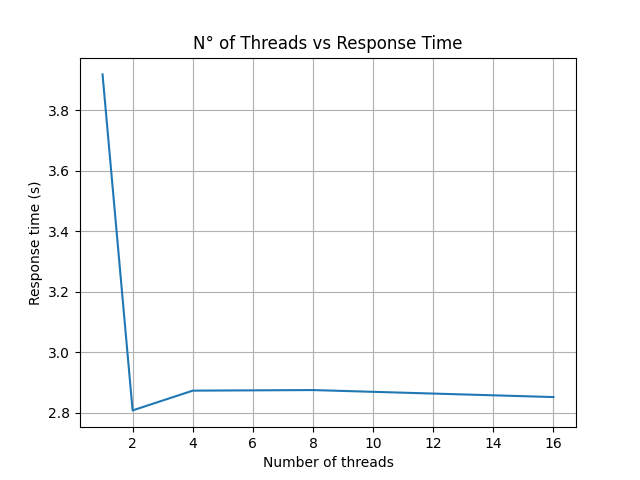
\includegraphics[width=0.4\textwidth]{../plots/4k_response_time.png}
    \caption{Gráfica de tiempos de respuesta para las ejecuciones de la aplicación del filtro sobre la imagen de tamaño 4k}
\end{figure}

En este caso se puede observar como los tiempos de ejecución son siempre decrecientes, a pesar de tener únicamente 6 núcleos, los tiempos se redujeron inclusive usando 16 hilos con lo que se puede inferir que los tiempos del sistema operativo pudieron interferir positivamente en estos últimos casos. Sin embargo es bastante notorio como el uso de múltiples hilos para el procesamiento de la imagen, redujeron los tiempos de procesamiento desde un poco mas de 2.2 segundos hasta 1.3 segundos en el mejor caso.

\begin{figure}[H]
    \centering
    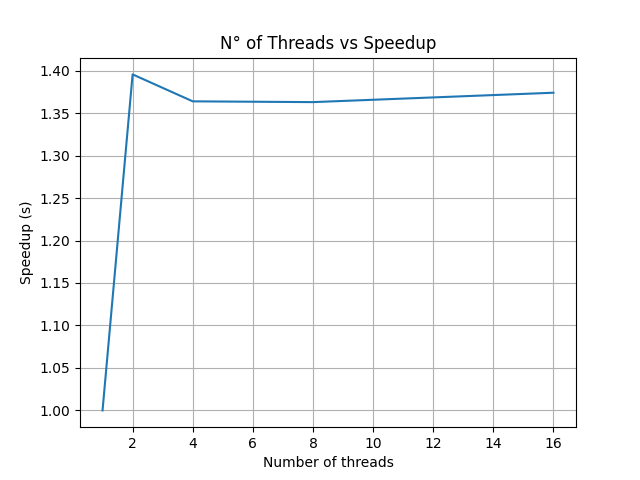
\includegraphics[width=0.4\textwidth]{../plots/4k_speedup.png}
    \caption{Gráfica de tiempos de respuesta para las ejecuciones de la aplicación del filtro sobre la imagen de tamaño 4k}
\end{figure}

En el caso del speed up, se puede notar como este siempre es positivo mostrando una notoria mejora cuando se aumenta el uso de núcleos para el procesamiento de la imagen.

\subsection{Imagen de tamaño 1080p}

La imagen obtenida de aplicar el filtro es la siguiente:

\begin{figure}[H]
    \centering
    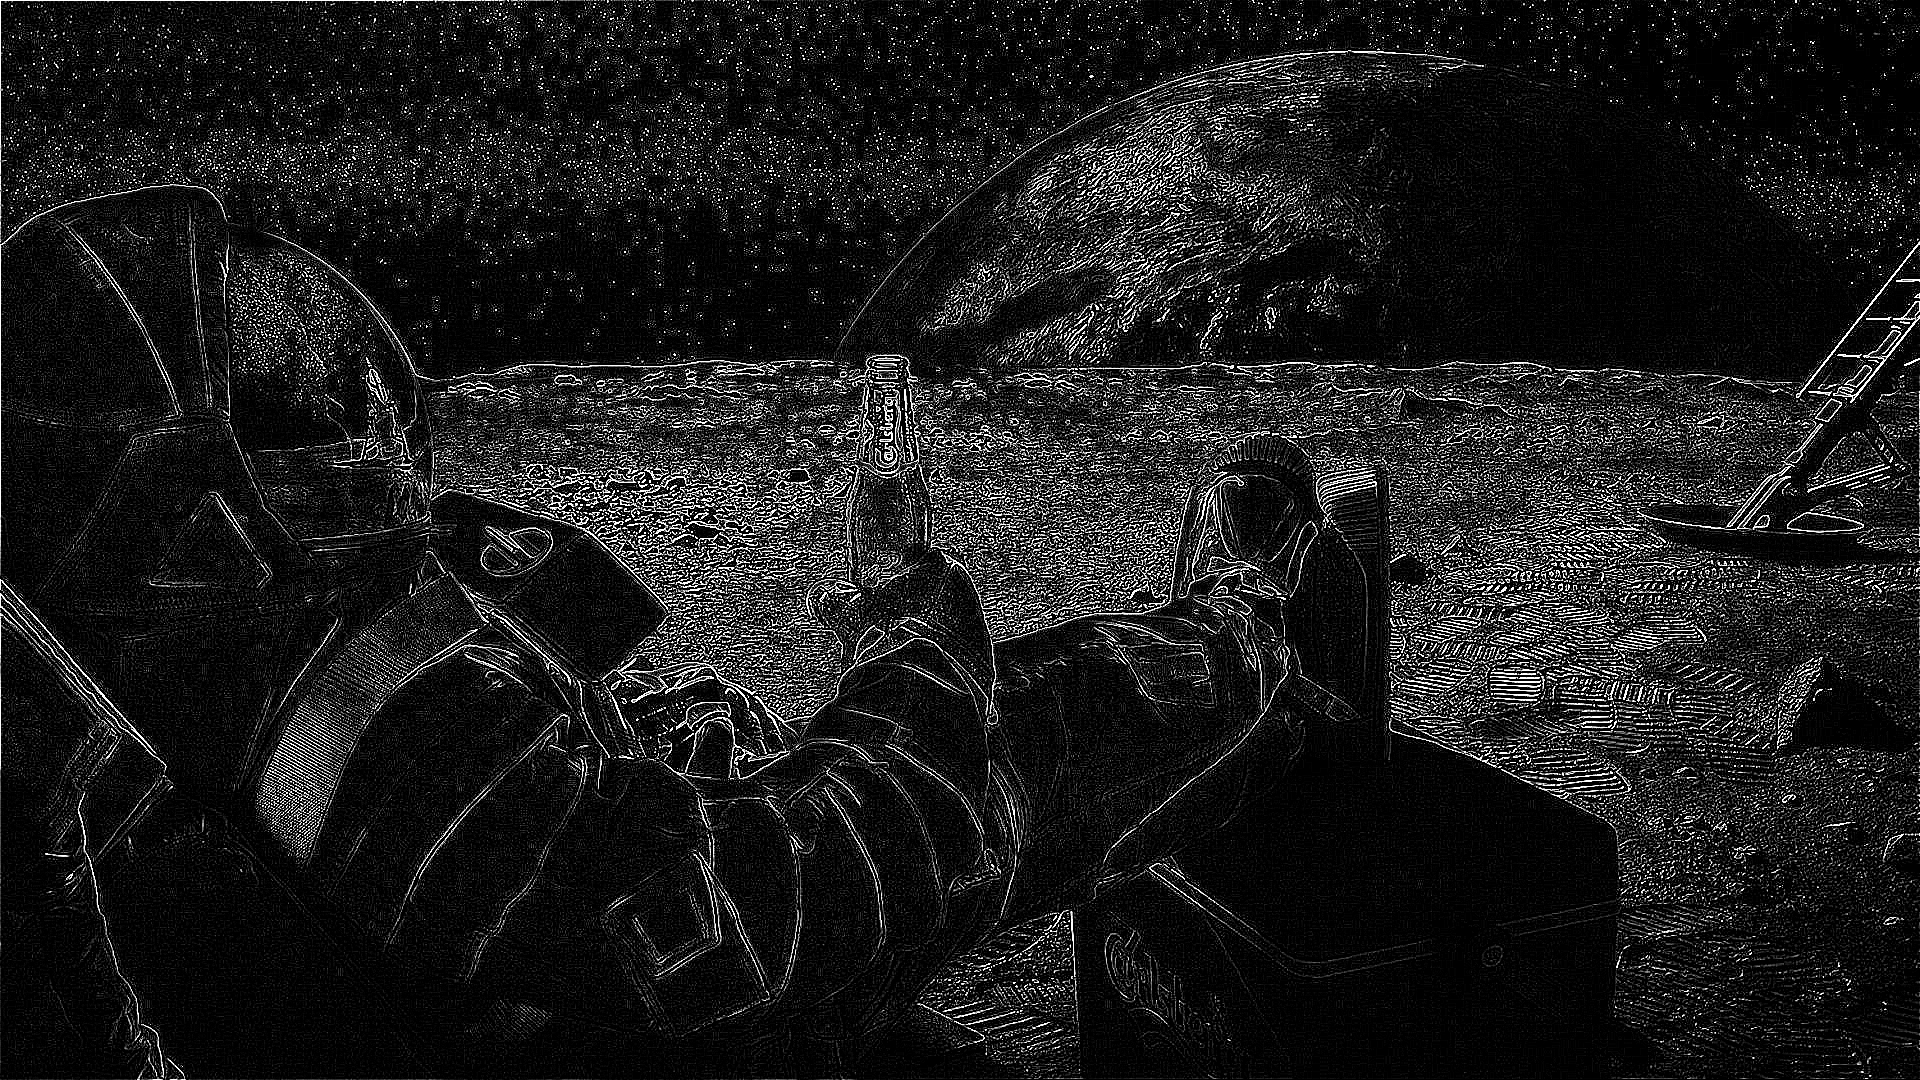
\includegraphics[width=0.4\textwidth]{../plots/1080p.out.jpg}
    \caption{Miniatura de imagen con tamaño 1080p con el filtro de detección de bordes aplicado.}
\end{figure}

Las gráficas que resumen y comparan los tiempo de respuesta y los speed up de la aplicación del filtro a esta imagen son los siguientes:

\begin{figure}[H]
    \centering
    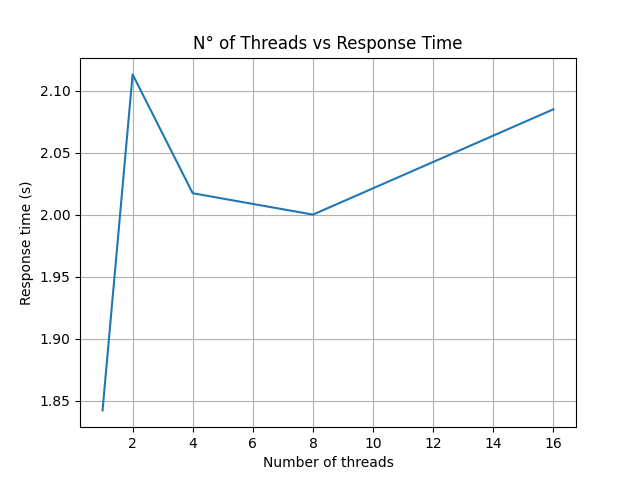
\includegraphics[width=0.4\textwidth]{../plots/1080p_response_time.png}
    \caption{Gráfica de tiempos de respuesta para las ejecuciones de la aplicación del filtro sobre la imagen de tamaño 1080p}
\end{figure}

En este caso llama la atención como en los casos de procesamiento con 8 y 16 núcleos los tiempos crecieron, esto se puede justificar en los 6 núcleos del procesador, en estos casos solo 6 hilos se ejecutaban al mismo tiempo mientras que los demás trabajaban su parte del filtro de manera concurrente.

\begin{figure}[H]
    \centering
    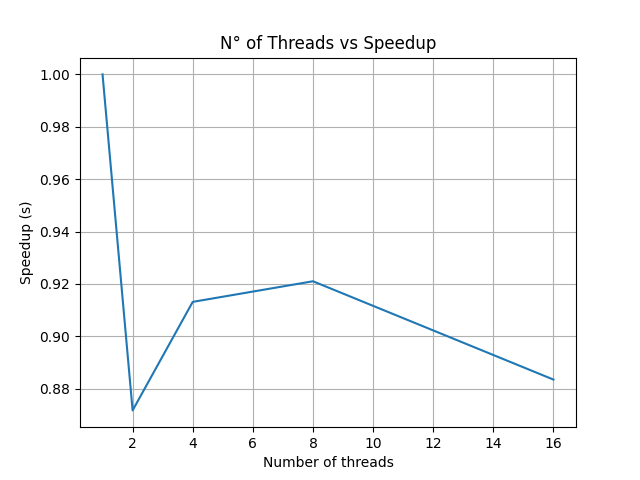
\includegraphics[width=0.4\textwidth]{../plots/1080p_speedup.png}
    \caption{Gráfica de tiempos de respuesta para las ejecuciones de la aplicación del filtro sobre la imagen de tamaño 1080p}
\end{figure}

De manera similar a los tiempos de respuesta, el resultado para 8 y 16 hilos es irregular y se puede asumir esto debido a los 6 núcleos del procesador. Algo a tener en cuenta es que el speed up en el caso de la imagen 4k fue muy similar al caso de 720p, esto se puede justificar en que independiente mente del tamaño de la imagen siempre se va a estar paralelizando la misma proporción de código.

\subsection{Imagen de tamaño 720p}

La imagen obtenida de aplicar el filtro es la siguiente:

\begin{figure}[H]
    \centering
    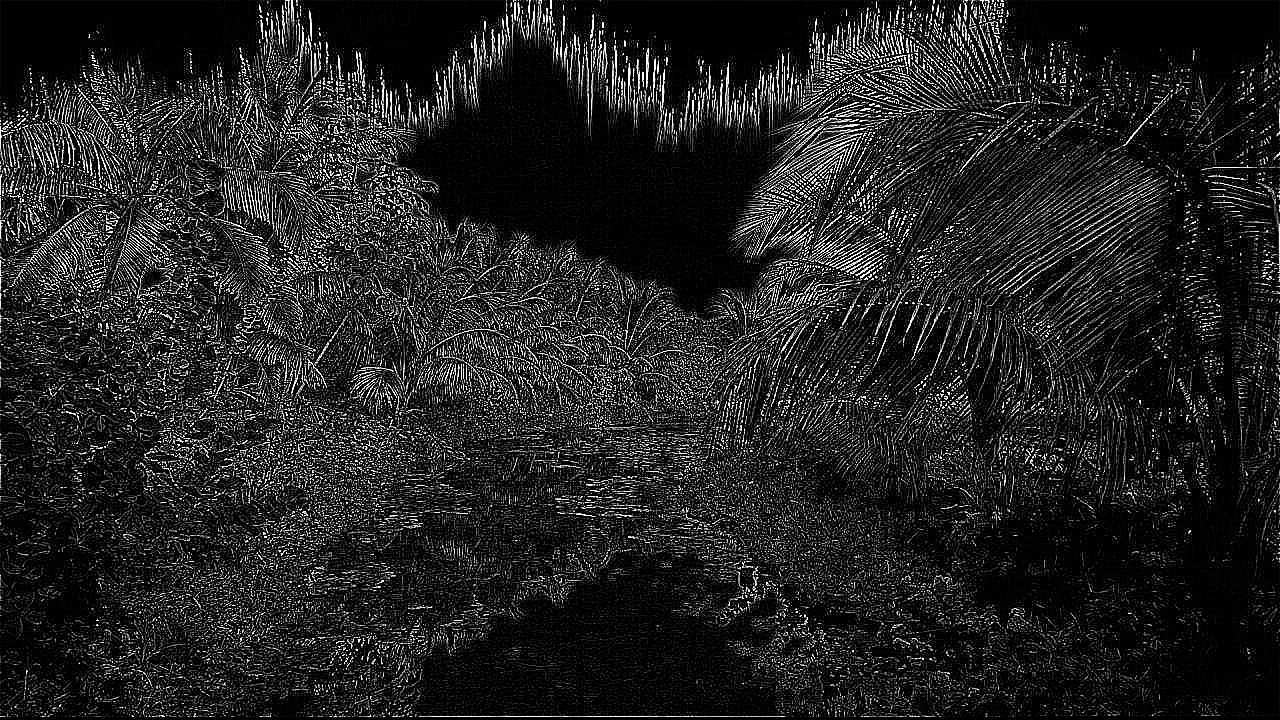
\includegraphics[width=0.4\textwidth]{../plots/720p.out.jpg}
    \caption{Miniatura de imagen con tamaño 720 con el filtro de detección de bordes aplicado.}
\end{figure}

Las gráficas que resumen y comparan los tiempo de respuesta y los speed up de la aplicación del filtro a esta imagen son los siguientes:

\begin{figure}[H]
    \centering
    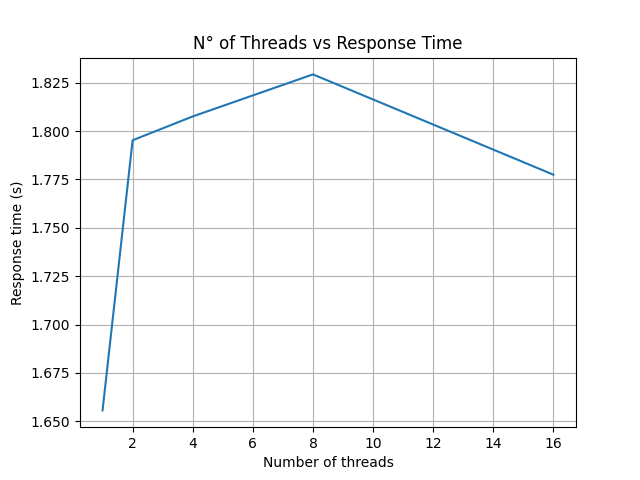
\includegraphics[width=0.4\textwidth]{../plots/720p_response_time.png}
    \caption{Gráfica de tiempos de respuesta para las ejecuciones de la aplicación del filtro sobre la imagen de tamaño 720p}
\end{figure}

En este caso nuevamente tenemos una irregularidad en las ejecuciones con 8 y 16 hilos que se justifican con los 6 núcleos del procesador, los tiempos de ejecución total del programa para tamaño 720p están en el orden de 100 ms, por lo que los tiempos del sistema operativo pueden estar interfiriendo con los resultados.

\begin{figure}[H]
    \centering
    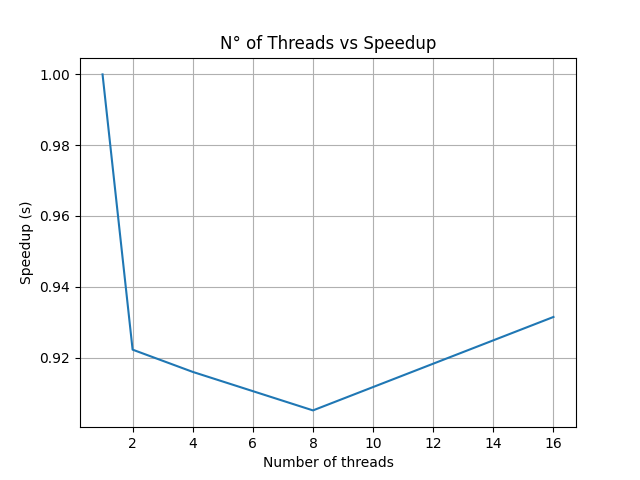
\includegraphics[width=0.4\textwidth]{../plots/720p_speedup.png}
    \caption{Gráfica de tiempos de respuesta para las ejecuciones de la aplicación del filtro sobre la imagen de tamaño 720p}
\end{figure}

Finalmente en este caso encontramos la irregularidad que ya se mencionó en las ejecuciones con 8 y 16 hilos, además notamos que nuevamente el speed up en los casos de 4 núcleos es muy similar al speed up en los casos de 4k y 1080p debido a que se paraleliza la misma proporción de código.

\section{Conclusiones}

\begin{itemize}
    \item La aplicación de filtros sobre imágenes son procesos altamente paralelizables debido a que cada proceso realizado sobre cada pixel es independiente de los demás.
    \item Las gráficas de speed up permiten identificar el límite de eficiencia que se puede alcanzar al paralelizar el algoritmo de detección de bordes. Estos resultados están sustentados bajo la ley de Amdahl, la cual establece un límite de speed up a medida que se aumenta el número de hilos usados en la ejecución.
    \item Los tiempos del sistema operativo afectan considerablemente los tiempos de ejecución de un programa cuando sus tiempos son muy cortos.
\end{itemize}

\end{document}
